
\documentclass[border=3pt,tikz]{standalone}
\usetikzlibrary{calc} % for calculating coordinates in \connect
\tikzset{>=latex}
\def\connect[#1] (#2)!#3!(#4){ % straight connector with two corners
  \draw[#1] (#2) |- ($(#2)!#3!(#4)$) node[pos=0.5] (#2-#4-1) {}
  -| (#4) node[pos=0.5] (#2-#4-2) {}
}
\begin{document}
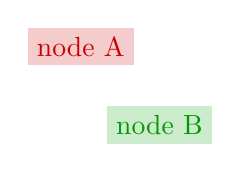
\begin{tikzpicture}
  \node[red!80!black,fill=red!80!black!20] (A) at (0,0) {node A};
  \node[green!60!black,fill=green!60!black!20] (B) at (1,-1) {node B};
  \connect[->,thick,red] (A)!0.4!(B);
\end{tikzpicture}
\end{document}
